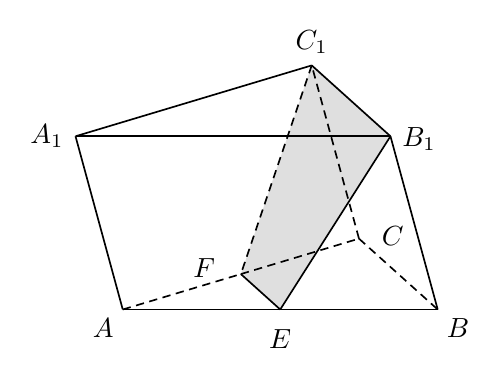
\begin{tikzpicture}[line width=0.6pt, font=\normalsize]
\coordinate (A) at (0,0);
\coordinate (B) at (4,0);
\coordinate (C) at (3.0,0.9);
\coordinate (E) at (2,0);
\coordinate (F) at (1.5,0.45);
\coordinate (A1) at (-0.6,2.2);
\coordinate (B1) at (3.4,2.2);
\coordinate (C1) at (2.4,3.1);
% section fill first (gray block keeps boundary)
\fill[gray!25] (F) -- (E) -- (B1) -- (C1) -- cycle;
% bottom face
\draw (A) -- (E) -- (B);
\draw[densely dashed] (A) -- (F);
\draw[densely dashed] (F) -- (C);
\draw[densely dashed] (C) -- (B);
% top face
\draw (A1) -- (B1);
\draw (B1) -- (C1);
\draw (A1) -- (C1);
% lateral edges
\draw (A) -- (A1);
\draw (B) -- (B1);
\draw[densely dashed] (C) -- (C1);
% section edges
\draw (F) -- (E);
\draw (E) -- (B1);
\draw[densely dashed] (C1) -- (F);
% labels
\node[fill=white,inner sep=1pt,anchor=north east] at ([shift={(-2pt,-2pt)}]A) {$A$};
\node[fill=white,inner sep=2pt,anchor=north] at ([shift={(0pt,-5pt)}]E) {$E$};
\node[fill=white,inner sep=1pt,anchor=north west] at ([shift={(2pt,-2pt)}]B) {$B$};
\node[fill=white,inner sep=2pt,anchor=west] at ([shift={(6pt,1pt)}]C) {$C$};
\node[fill=white,inner sep=2pt,anchor=east,fill=none,xshift=-2.00bp,yshift=0.00bp] at ([shift={(-5pt,2pt)}]F) {$F$};
\node[fill=white,inner sep=1pt,anchor=east] at ([shift={(-3pt,0pt)}]A1) {$A_{1}$};
\node[fill=white,inner sep=1pt,anchor=west] at ([shift={(3pt,-1pt)}]B1) {$B_{1}$};
\node[fill=white,inner sep=1pt,anchor=south] at ([shift={(0pt,3pt)}]C1) {$C_{1}$};
\end{tikzpicture}
